%%%%%%%%%%%%%%%%%%%%%%%%%%%%%%%%%%%%%%%%%
% Jacobs Landscape Poster
% LaTeX Template
% Version 1.1 (14/06/14)
%
% Created by:
% Computational Physics and Biophysics Group, Jacobs University
% https://teamwork.jacobs-university.de:8443/confluence/display/CoPandBiG/LaTeX+Poster
% 
% Further modified by:
% Nathaniel Johnston (nathaniel@njohnston.ca)
%
% This template has been downloaded from:
% http://www.LaTeXTemplates.com
%
% License:
% CC BY-NC-SA 3.0 (http://creativecommons.org/licenses/by-nc-sa/3.0/)
%
%%%%%%%%%%%%%%%%%%%%%%%%%%%%%%%%%%%%%%%%%

%----------------------------------------------------------------------------------------
%	PACKAGES AND OTHER DOCUMENT CONFIGURATIONS
%----------------------------------------------------------------------------------------

\documentclass[final]{beamer}

\usepackage[scale=1.24]{beamerposter} % Use the beamerposter package for laying out the poster
\usepackage{multicol}

\usetheme{confposter} % Use the confposter theme supplied with this template

\setbeamercolor{block title}{fg=ngreen,bg=white} % Colors of the block titles
\setbeamercolor{block body}{fg=black,bg=white} % Colors of the body of blocks
\setbeamercolor{block alerted title}{fg=white,bg=dblue!70} % Colors of the highlighted block titles
\setbeamercolor{block alerted body}{fg=black,bg=dblue!10} % Colors of the body of highlighted blocks
% Many more colors are available for use in beamerthemeconfposter.sty

%-----------------------------------------------------------
% Define the column widths and overall poster size
% To set effective sepwid, onecolwid and twocolwid values, first choose how many columns you want and how much separation you want between columns
% In this template, the separation width chosen is 0.024 of the paper width and a 4-column layout
% onecolwid should therefore be (1-(# of columns+1)*sepwid)/# of columns e.g. (1-(4+1)*0.024)/4 = 0.22
% Set twocolwid to be (2*onecolwid)+sepwid = 0.464
% Set threecolwid to be (3*onecolwid)+2*sepwid = 0.708

\newlength{\sepwid}
\newlength{\onecolwid}
\newlength{\twocolwid}
\newlength{\threecolwid}
% MAX DIMENSIONS FOR COG SCI 96 x 48
\setlength{\paperwidth}{60in} % A0 width: 46.8in
\setlength{\paperheight}{42in} % A0 height: 33.1in
\setlength{\sepwid}{0.03\paperwidth} % Separation width (white space) between columns
\setlength{\onecolwid}{0.25\paperwidth} % Width of one column
\setlength{\twocolwid}{0.35\paperwidth} % Width of two columns
\setlength{\threecolwid}{0.708\paperwidth} % Width of three columns
\setlength{\topmargin}{-0.5in} % Reduce the top margin size
%-----------------------------------------------------------

\usepackage{graphicx}  % Required for including images

\usepackage{booktabs} % Top and bottom rules for tables

%----------------------------------------------------------------------------------------
%	TITLE SECTION 
%----------------------------------------------------------------------------------------

\title{Efficiency of Learning in Experience-Limited Domains:\\Generalization Beyond the WUG Test} % Poster title

\author{Christopher~R. Cox$^1$, Matthew Cooper~Borkenhagen$^2$ and Mark~S. Seidenberg$^2$} % Author(s)

\institute{1. Louisiana State University, 2. University of Wisconsin-Madison} % Institution(s)

%----------------------------------------------------------------------------------------

\begin{document}

\addtobeamertemplate{block end}{}{\vspace*{2ex}} % White space under blocks
\addtobeamertemplate{block alerted end}{}{\vspace*{2ex}} % White space under highlighted (alert) blocks

\setlength{\belowcaptionskip}{2ex} % White space under figures
\setlength\belowdisplayshortskip{2ex} % White space under equations

\begin{frame}[t] % The whole poster is enclosed in one beamer frame

\begin{columns}[t] % The whole poster consists of three major columns, the second of which is split into two columns twice - the [t] option aligns each column's content to the top

\begin{column}{\sepwid}\end{column} % Empty spacer column

\begin{column}{\onecolwid} % The first column

%----------------------------------------------------------------------------------------
%	OBJECTIVES
%----------------------------------------------------------------------------------------
\begin{alertblock}{Introduction}

\begin{itemize}
    \item \textbf{Generalization}---the ability to apply existing knowledge to novel cases---is essential for language acquisition and learning to read.
    \item Nonce words that do not occur in natural speech like NUST or GLORP can be read aloud \cite{Seidenberg1989}.
    \item Children's vocabulary development depends on their exposure to spoken language, which varies considerably \cite{Hart1995,Gilkerson2017} with enormous consequences for learning to read and other aspects of schooling.
    \item Knowledge gaps cannot be closed solely through explicit instruction because there isn't sufficient classroom time.
    \item \textbf{Our research examined the relation between generalization and efficiency of learning.}
\end{itemize}
\end{alertblock}

\begin{figure}[h]
  \centering
  \def\svgwidth{0.7\linewidth}
  \input{figures/WUG-test-2.pdf_tex}
  \caption{The WUG Test \cite{Berko1958}. When presented with a novel noun, even young children will generalize the plural ``s'' when speaking about more than one of them.}
  \label{fig:wug}
\end{figure}

%----------------------------------------------------------------------------------------
\begin{block}{Approach}
  \begin{itemize}
    \item Children need to generate pronunciations for many written words (the target set);
    \item They are explicitly taught the correspondences between orthography and phonology for a much smaller subset of words (the training set);
    \item Generalization is assessed in terms of correct performance on untrained items from the target set, rather than nonce forms. \textbf{This shifts the focus of generalization to acquiring real-world knowledge.}
  \end{itemize}

  \vspace{1em}
    \textbf{We examined efficiency of learning as a function of training set size using well-studied models of learning orthography-phonology correspondences \cite{Seidenberg1989,Harm1999}.}
\end{block}

\begin{block}{Model training and evaluation}
One million models were run, 100k with each of 10 training set sizes $(100,200,\dots,1000)$ comprised of words sampled randomly without replacement from the 2881 word target set.
Each model was trained for 3000 weight updates with a constant learning rate $(\eta=0.1)$.
The model was exposed to the whole training set before each update.
Each model was then tested on the untrained remainder of the target corpus to evaluate generalization.
An output pattern was scored as correct if all unit activations were within 0.5 of their target state.
\end{block}

\end{column} % End of the first column

\begin{column}{\sepwid}\end{column} % Empty spacer column

\begin{column}{\twocolwid} % Begin a column which is two columns wide (column 2)

%----------------------------------------------------------------------------------------
%	MATERIALS
%----------------------------------------------------------------------------------------
\setbeamercolor{block alerted title}{fg=white,bg=norange} % Change the alert block title colors
\setbeamercolor{block alerted body}{fg=black,bg=white} % Change the alert block body colors
\begin{alertblock}{Conclusion}
  \begin{center}
    \item It is possible to be more efficient with curricula that attend to the number of words taught and the words that are prioritized in teaching.
  \vspace{0.75em}
  \end{center}
\end{alertblock}

\begin{block}{Model Performance}

\begin{figure}[h]
  \centering
  \def\svgwidth{1.0\linewidth}
  \input{figures/generalization_vioplot_wide.pdf_tex}
  \caption{Summary of model performance as a function of the size of the training set.}
  \label{fig:generalization}
\end{figure}

\begin{columns}[t]
  \begin{column}{0.58\linewidth}
    \begin{figure}[h]
      \centering
      \def\svgwidth{0.9\linewidth}
      \input{figures/word_accuracy_over_testsets.pdf_tex}
      \caption{ The probability that each word would be accurately generalized to, given that it was not trained on, summarized in a histogram. A random selection of words in each bin are printed.}
      \label{fig:word_acc}
    \end{figure}

  \end{column}

  \begin{column}{0.04\linewidth}
  \end{column}

  \begin{column}{0.38\linewidth}
    \begin{figure}[h]
      \centering
      %\def\svgwidth{0.9\linewidth}
      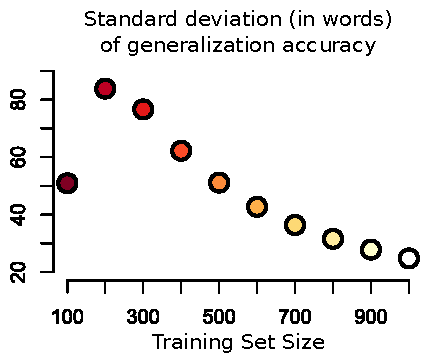
\includegraphics[width=1.0\linewidth]{figures/generalization_std_colored_embedded_fonts.pdf}
      \caption{Standard deviation of generalization accuracy over the 100k models fit at each training set size.}
      \label{fig:generalization_std}
    \end{figure}

  \end{column}
\end{columns}

\end{block}

\begin{block}{Predicting generalizability}

\begin{columns}[t]
  \begin{column}{0.34\linewidth}
    \vspace{-1.1em}
    \begin{table}[t]
      \small
      \begin{tabular}{r r r r r}
       & \textbf{WL} & \textbf{ON} & \textbf{PN} & \textbf{Con.} \\
       \toprule
        \textit{Word Length}          &  1.00 & & & \\
        \textit{Orth. Neighbors}      & -0.65 &  1.00 & & \\
        \textit{Phon. Neighbors}      & -0.28 &  0.35 &  1.00 & \\
        \textit{Consistency}          & -0.03 & -0.02 & -0.02 & 1.00 \\
        \midrule
        \textit{P(accuracy)}          & -0.27  & 0.47 & 0.28 & 0.38 \\
      \end{tabular}
      \caption{Correlation among lexical variables. Bottom row shows each variable correlated with probability of accuracy.}
      \label{tab:cormat}
    \end{table}
  \end{column}

  \begin{column}{0.01\linewidth} \end{column}

  \begin{column}{0.32\linewidth}
    \begin{table}[t]
      \small
      \begin{center}
        \begin{tabular}{r r r r r}
          \textbf{Word Level} & $\eta^2_p$ & $\Delta \mathbf{R^2}$ \\
          \toprule
          \textit{Word length}       & 0.01 & 0.00 \\
          \textit{Orth. Neighbors}   & 0.17 & 0.13 \\
          \textit{Phon. Neighbors}   & 0.03 & 0.02 \\
          \textit{Consistency}       & 0.20 & 0.15 \\
          \bottomrule

        \end{tabular}
        \caption{Effect sizes describing the variance explained by regressing the probability of accurately generalizing to an untrained word on several variables.}
        \label{tab:effectsize}
      \end{center}
    \end{table}
  \end{column}

  \begin{column}{0.01\linewidth} \end{column}

  \begin{column}{0.32\linewidth}
    \begin{table}
      \small
      \begin{center}
        \begin{tabular}{r r r}
          \textbf{Model Level} & $\eta^2_p$ & $\Delta \mathbf{R^2}$ \\
          \toprule
          \textit{Word length}       & 0.002 & 0.001 \\
          \textit{Orth. Neighbors}   & 0.006 & 0.005 \\
          \textit{Phon. Neighbors}   & 0.000 & 0.000 \\
          \textit{Consistency}       & 0.137 & 0.136 \\
          \bottomrule
        \end{tabular}
        \caption{Effect sizes describing the variance explained by regressing generalization accuracy on aggregate training set stats.}
        \label{tab:effectsize_model}
      \end{center}
    \end{table}

  \end{column}
\end{columns}
%----------------------------------------------------------------------------------------

\end{block}
\end{column} % End of the second column

\begin{column}{\sepwid}\end{column} % Empty spacer column

\begin{column}{\onecolwid} % The third column

\begin{block}{Target words}

The simulations used a set of \textbf{2881 monosyllabic English} words employed in previous research \cite{Harm1999}.
Word length ranged from 2--8 letters and 1--7 phonemes.
Words were presented uniformly, ignoring frequency in natural language.

\end{block}

\begin{block}{Model architecture and word representations}
Feedforward network with an input orthographic layer (102 units), an output phonological layer (66 units) and a single hidden layer (100 units).
Weights updated with gradient descent and backpropagation after accumulating cross-entropy error over all words in the training set.
The model was implemented using scikit-learn in Python 3.6 using a multilayer perceptron, and training was executed in parallel using HTCondor \cite{Thain2005} and computational resources maintained by the Center for High Throughput Computing at UW Madison.

\vspace{1em}

\begin{columns}[t]
  \small
  \begin{column}{0.48\linewidth}
  \textbf{Orthographic representations were generated as follows:}
  \begin{enumerate}
    \item Words were vowel-centered and padded with ``empty letters'' to establish uniform length (14 letters).
    \item The letter \textit{y} was treated as a consonant when it began a word and a vowel otherwise.
    \item Each letter was represented by one unit in a 26 element vector.
    \item Vectors were condensed by eliminating nodes for unused features, resulting in an input layer with 102 features.
  \end{enumerate}
  \end{column}
  \begin{column}{0.04\linewidth}
  \end{column}
  \begin{column}{0.48\linewidth}
    \textbf{Phonological word forms were represented using 41 phonemes (26 consonants, 15 vowels):}
  \begin{enumerate}
    \item They were aligned on the first vowel, adding empty phonemes at the beginning or end to produce phonological representations of equal length (10 phonemes including empty phonemes).
    \item Each phoneme was defined by 25 phonetic features \cite{Harm1999}.
    \item Vectors were condensed by eliminating nodes for unused features, resulting in an output layer with 66 features.
  \end{enumerate}
  \end{column}
\end{columns}

\end{block}



%----------------------------------------------------------------------------------------
%	REFERENCES
%----------------------------------------------------------------------------------------

\begin{block}{References}

%\nocite{*} % Insert publications even if they are not cited in the poster
\begin{multicols}{2}
\scriptsize{\bibliographystyle{unsrt}
\bibliography{CogSci_2019_CoxCooperBorkenhagenSeidenberg.bib}\vspace{0.75in}}
\end{multicols}

\end{block}

%----------------------------------------------------------------------------------------
%	ACKNOWLEDGEMENTS
%----------------------------------------------------------------------------------------

\setbeamercolor{block title}{fg=red,bg=white} % Change the block title color

\begin{block}{Acknowledgements}

\small{\rmfamily{This work has been supported by the Vilas Trust at UW-Madison and by the Institute of Education Sciences, US Department of Education, through Award R305B150003 to UW-Madison. The opinions expressed are those of the authors and do not represent views of the US Department of Education.}}\\
\end{block}

%----------------------------------------------------------------------------------------
%	CONTACT INFORMATION
%----------------------------------------------------------------------------------------

%\setbeamercolor{block alerted title}{fg=black,bg=norange} % Change the alert block title colors
%\setbeamercolor{block alerted body}{fg=black,bg=white} % Change the alert block body colors
%
%\begin{alertblock}{Contact Information}
%
%\begin{itemize}
%\item Web: \href{http://www.university.edu/smithlab}{http://www.university.edu/smithlab}
%\item Email: \href{mailto:john@smith.com}{john@smith.com}
%\item Phone: +1 (000) 111 1111
%\end{itemize}
%
%\end{alertblock}
%
%\begin{center}
%\begin{tabular}{ccc}
%\includegraphics[width=0.4\linewidth]{logo.png} & \hfill & \includegraphics[width=0.4\linewidth]{logo.png}
%\end{tabular}
%\end{center}

%----------------------------------------------------------------------------------------

\end{column} % End of the third column

\end{columns} % End of all the columns in the poster

\end{frame} % End of the enclosing frame

\end{document}
